%%=============================================================================
%% Methodologie
%%=============================================================================


\chapter{\IfLanguageName{dutch}{Methodologie}{Methodology}}
\label{ch:methodologie}


Rekeninghoudend met de bevindingen uit de literatuurstudie, zal hier verder besproken worden hoe we een systeem gaan opstellen dat gepaste aanbevelingen kan maken. Gezien we twee verschillende werkwijzen en technologieën zullen vergelijken, zal voor beide systemen een werkwijze voorgesteld worden. Deze werkwijze zal ook in dit hoofdstuk verder uitgewerkt worden.

\section{Uitwerking ElasticSearch}
\label{sec:Uitwerking ElasticSearch}

Voor de uitwerking van Elasticsearch wordt een instantie opgezet waarmee we zullen communiceren, op deze instantie draait Elasticsearch. 

In Elasticsearch worden items opgeslagen als een document met enkele waarden, typisch aan een product. In dit onderzoek zijn deze waarden; 'naam', 'merk', 'categorieën', en 'prijs'. 

\subsection{Producten}
\label{sec:Producten}
Voor het aanmaken van de product data zullen enkele query's uitgevoerd worden die er als volgt uitzien:

\newpage
\begin{lstlisting}[caption={Query om één enkel product aan te maken},captionpos=b]
POST http://35.233.112.106:9200/products/product/1 
{ 
 "name": "Logitech G930",
 "brand": "Logitech",
 "categories": ["Headset", "Wireless headset", "Headphones"],
 "price": "190.00"
}
\end{lstlisting}

Op deze manier worden enkele producten in de databank gezet, met enkele verwante velden zoals gelijkaardige categorieën, zodat we hiermee aanbevelingen kunnen maken. Deze verzameling van producten wordt een index genoemd.

Vervolgens kunnen we een zoekterm ingeven via volgende query, deze zal alle resultaten weergeven waarvan een van de velden voldoet aan de meegegeven waarde, namelijk "deodorant". 

\begin{lstlisting}[caption={Query om één enkel product op te halen},captionpos=b]
GET http://35.233.112.106:9200/products/product/1 
{
 "query" : {
  "query_string": {
   "query": "deodorant"
  }
 }
}
\end{lstlisting}

\subsection{Gebruikers}

Er zullen enkele vooraf gedefinieerde gebruikers opgesteld worden, waarmee bepaald zal worden of de zoekresultaten aan de verwachtingen voldoen. Een voorbeeld van een gebruiker is te zien in volgende query:
\begin{lstlisting}[caption={Query om één enkele gebruiker aan te maken}]
POST http://35.233.112.106:9200/users/user/1
{
	"name": "Louise",
	"age": "21",
	"address": {
		"city": "Aalst",
		"street": "Molendries 4",
		"province": "Oost-Vlaanderen"
	},
	"categories": ["Electronics, Apple"],
	"searches": ["iphone", "deodorant", "uncommon product"],
	"brands": ["Nivea", "Apple"]
}
\end{lstlisting}

Bij deze gebruiker kunnen we bijvoorbeeld verwachten dat als deze 'deodorant' opzoekt, zij die van het merk Nivea bovenaan de resultaten zal zien. 

Een voorbeeld van zo'n zoekopdracht, waarbij sommige velden ingevuld zijn op basis van onze persoon van de query hierboven, gaat als volgt:

\begin{lstlisting}[caption={Query om een zoekopdracht met term 'Deodorant' uit te voeren, met filters en een score op basis van informatie van een gebruiker}]
POST http://35.233.112.106:9200/products/_search
{
  "query": {
    "function_score": {
      "query": {
        "query_string": {
          "query": "Deodorant"
        }
      },
      "functions": [
        { "filter" : 
          { "terms" : 
            { "brand" : ["Niveau", "Apple"]  } 
          },
          "weight": 3
        },
        { "filter" : 
          { "terms" : 
            { "categories" : ["Electronics", "Apple"] }
          },
          "weight": 2
        },
        { "filter" : 
          { "terms" : 
            { "searches" : ["iphone", "deodorant", "uncommon product"] } 
          },
          "weight": 1
        }
      ],
      "score_mode": "sum",
      "boost_mode": "replace"
      }
   }
}
\end{lstlisting}

In het bovenste deel van de query, waar de \textit{query\textunderscore string} wordt aangeduid. Deze string zou dan overeenkomen met wat een gebruiker zou invoeren in een zoekbalk op een website.

In de realiteit zal de informatie over 'brand', 'categories', en 'searches' opgehaald worden uit het model van de persoon in kwestie.

In deze query wordt een score toegekend aan de resultaten die voldoen aan bovenstaande verwachting, namelijk dat het woord 'deodorant' terug te vinden moet zijn in een van de velden van het product (naam, merk, categorie)

\newpage
Die score wordt toegekend op basis van de informatie over een persoon, hieruit verstaan we dat dit gaat over de merken die deze persoon reeds gekocht heeft, in welke categorieën deze persoon reeds gekocht heeft, en een historiek van zoekopdrachten. Deze hebben elk een gewicht toegekend gekregen, respectievelijk drie, twee en één. 

In de query zijn drie filters te zien die de score van een resultaat zullen beïnvloeden. Bij elk van deze filters wordt het score vermenigvuldigd met het gewicht. \textit{score\textunderscore mode : sum} zorgt ervoor dat de resultaten van de scores opgeteld worden.

\textit{boost\textunderscore mode : replace} zorgt ervoor dat de score die verkregen wordt bij het gelijkaardig zijn aan de zoekterm vervangen wordt door de nieuw berekende score van de functies.

Deze query is een vorm van collaborative filtering, toegepast op zichzelf. De query zal dus gaan zoeken naar hoe verwant een resultaat is aan een persoon, op basis van enkele variabelen, en zal deze een hogere score toekennen afhankelijk van hoe relevant het product is voor een gebruiker. Resultaten met een hogere score zullen dus bijgevolg ook hoger in de lijst van resultaten komen te staan.

\subsection{Graph API Plug-in}
\label{sec:Graph API Plug-in}

Elasticsearch biedt ook een plug-in aan die de functionaliteiten van een graph database voorziet. Met deze plug-in bekomen we dus eigenlijk een Knowledge Graph zoals eerder in de literatuurstudie vermeld werd. 

Deze plug-in laat toe om connecties te vinden tussen objecten in de databank, en wordt geadverteerd als ook bruikbaar te zijn voor aanbevelingen.

Jammer genoeg is deze plug-in enkel beschikbaar wanneer we beschikken over een Platinum of Enterprise licentie. Door deze vereiste valt deze functionaliteit dus buiten de scope van het onderzoek. 

\begin{figure} [ht]
	\centering
	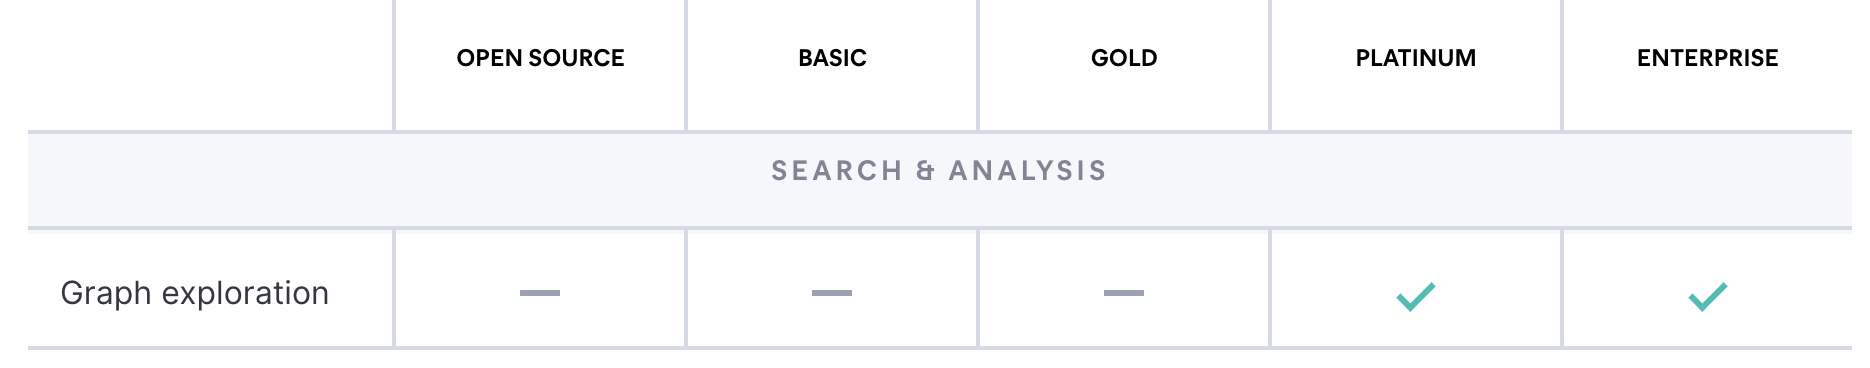
\includegraphics[width=0.95\textwidth]{img/elastic-license}
	\caption{Overzicht van de beschikbaarheid van de Graph plugin voor de Elastic licenties}
	\floatfoot{Source: https://www.elastic.co/subscriptions}
	\label{fig:elastic licenties overzicht graph}
\end{figure}

\newpage
\section{Uitwerking Neo4j}
\label{sec:UItwerking Neo4j}

Voor dit systeem wordt er een model opgesteld in een Graph databank, de gekozen technologie hiervoor is Neo4j. Op deze databank kunnen dan zoekalgoritmen uitgevoerd worden, om zo tot correcte aanbevelingen te komen. In dit hoofdstuk zal verder uitgewerkt worden hoe dit precies in elkaar zit.

\subsection{Model}
\label{sec:Model}
Relaties tussen producten en klanten zullen als volgt worden opgeslagen in deze Graph databank:

Er zijn 2 soorten nodes, dit zijn de knopen van een graaf, namelijk 'Gebruiker' en 'Product'. De relaties, aangeduid door lijnen tussen de knopen, zullen dan voorstellen wat de interactie van een gebruiker met een product is. Dit kan 'LIKES', 'BOUGHT', of 'LIVES\_TOGETHER' zijn. 'LIVES\_TOGETHER' zal dan aanduiden of 2 gebruikers familie of samenwonend zijn. 

De attributen van een Product zijn als volgt:
\begin{itemize}
	\item Product ID
	\item Name
	\item Brand
\end{itemize}

De attributen voor een Gebruiker zijn als volgt:
\begin{itemize}
	\item Name
	\item Address
\end{itemize}

De verschillende soorten relaties zijn als volgt:
\begin{itemize}
	\item 'BOUGHT' -> Gebruiker heeft Product gekocht
	\item 'LIKES' -> Gebruiker heeft Product leuk gevonden
	\item 'LIVES\_TOGETHER' -> Gebruiker 1 heeft hetzelfde adres als Gebruiker 2
\end{itemize}

Volgende query wordt gebruikt om de product- en klant nodes aan te maken, dit is uiteraard een verkorte versie:

\begin{lstlisting}[caption={Neo4j query voor het aanmaken van producten en klanten}]
CREATE 
(shauni:Customer {name: 'Shauni', address: 'Exterkenstraat 14'}),
(lynn:Customer {name: 'Lynn', address: 'Exterkenstraat 14'}),
(angelo:Customer {name: 'Angelo', address: 'Arbeidstraat 14'}), 
...
(prod1:Product{id: '1', name:'Hairbrush', brand:'Syoss'}), 
(prod2:Product{id: '2', name:'Instant Chocolate Milk', brand:'Nesquick'}), 
(prod3:Product{id: '3', name:'Toilet Paper', brand: 'Boni'}), 
...
\end{lstlisting}

Om een relatie aan te maken tussen een product en een gebruiker zal volgende query gebruikt worden. Deze zal dus uitgevoerd worden elke keer een gebruiker een actie uitvoert met een product.
Aangezien een product leuk vinden en een product kopen niet aanzien worden als evenwaardig, zullen er gewichten toegekend worden aan de interacties tussen gebruikers en producten.  Dat kan door middel van volgende query:

\begin{lstlisting}[caption={Neo4j query voor het aanmaken van een relatie tussen een product en een klant}]
	MATCH (c:Customer),(p:Product) 
	WHERE c.name = 'Shauni' AND p.id=3 
	CREATE (c)-[r:BOUGHT]->(p) 
	SET r.score = 3
\end{lstlisting}

Een product leuk vinden krijgt een score 2 toegekend, en een product kopen zal de score 3 krijgen, om de relatie 'LIKES' aan te maken zal in bovenstaande query de relatie 'BOUGHT' en de score moeten aangepast worden.

Om de relatie van Gebruikers die op eenzelfde adres wonen aan te maken, gebruiken we volgende query: 

\begin{lstlisting}[caption={Neo4j query voor het aanmaken van een relatie tussen een twee klanten.}]
	MATCH (a:Customer), (b:Customer) 
	WHERE EXISTS (a.address) AND EXISTS (b.address) AND a.address=b.address AND id(a)<id(b) 
	CREATE (a)-[:LIVES\_TOGETHER]->(b); 
\end{lstlisting}

De uiteindelijke graaf die voor dit zeer klein voorbeeld opgebouwd werd, zal al snel een beter inzicht geven in hoe deze data aan elkaar vast hangt. Dit is ook een van de troeven van Neo4j, het voorstellen van duidelijke visuele beelden die het eenvoudig maken om te begrijpen wat er zich op de achtergrond afspeelt. De graaf is te zien in Figuur \ref{fig:neo4jfullgraph}
\newpage

\begin{figure} [h!]
	\centering
	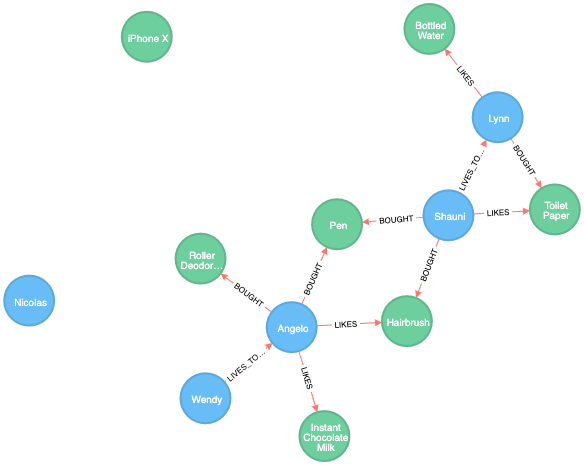
\includegraphics[width=0.95\textwidth]{img/full_graph_result}
	\caption{Overzicht van de ingevoerde data in een Neo4j graaf}
	\label{fig:neo4jfullgraph}
\end{figure}


\subsection{Ophalen van data}
\label{sec:Neo4j Ophalen van data}

Voor deze uitwerking werden enkele query's opgesteld die op basis van de relaties producten retourneren die zouden kunnen dienen als aanbevelingen.

Zo kan er bijvoorbeeld een lijst van producten gegenereerd worden die leuk gevonden of gekocht werden door de familieleden van een bepaalde gebruiker, dit gebeurt op basis van de relatie LIVES\_TOGETHER.

\begin{lstlisting}[caption={Neo4j query die alle likes en aankopen van de familie van een bepaalde gebruiker c1 weergeeft}]
MATCH (c1: Customer)
WHERE c1.name = 'Shauni'
MATCH (c1) - [:LIVES_TOGETHER] -> (c2 : Customer) - [:BOUGHT] -> (p:Product)
RETURN p as Product
UNION
MATCH (c1) - [:LIVES_TOGETHER] -> (c2) - [:LIKES] -> (p:Product)
RETURN p as Product
\end{lstlisting}

Ook van belang is het ophalen van producten die gebruikers kopen waar een gebruiker \textit{c1} gemeenschappelijke aankopen mee heeft. Dit kan via volgende query:

\begin{lstlisting}[caption={Neo4j query die de aankopen van gebruikers weergeeft waar een gebruiker c1 gemeenschappelijke aankopen mee heeft}]
MATCH (c1: Customer)
WHERE c1.name = 'Shauni'
MATCH(c1) - [:BOUGHT] -> (p1 : Product) <- [:BOUGHT] - (c2: Customer) - [:BOUGHT] -> (p2: Product)
RETURN p2
\end{lstlisting}

Om ditzelfde te bereiken maar dan inclusief de likes van deze gebruikers waar een gebruiker \textit{c1} gemeenschappelijke aankopen mee heeft, kan volgende query gebruikt worden: 

\begin{lstlisting}[caption={Neo4j query die de aankopen en likes van gebruikers weergeeft waar een gebruiker c1 gemeenschappelijke aankopen mee heeft}]
MATCH (c1) - [:BOUGHT] -> (p1 : Product) <- [:BOUGHT] - (c2: Customer) - [:BOUGHT] -> (p2: Product)
RETURN p2 as Product
UNION ALL
MATCH (c1) - [:BOUGHT] -> (p1) <- [:BOUGHT] -(c2) - [:LIKES] -> (p2) 
WHERE id(c1)<id(c2)
RETURN p2 as Product
\end{lstlisting}


\subsection{Search}
\label{subsec: Search Neo4j}

Binnen neo4j is het ook mogelijk om zoekopdrachten uit te voeren op basis van een tekstveld. Hiervoor moet op voorhand een index aangemaakt worden waarin beschreven staat welke attributen van welke types van nodes gebruikt mogen worden om de ingevoerde tekst mee te vergelijken.

\begin{lstlisting}[caption={Een index creëren binnen Neo4j om zoekopdrachten op basis van tekst uit te voeren}]
CALL db.index.fulltext.createNodeIndex("namesAndBrands",["Product"],["name", "brand"])
\end{lstlisting}

In dit voorbeeld gebruiken we de attributen \textit{name} en \textit{brand} van het nodetype \textit{Product}, en nemen we als zoekterm ``deodorant``.  Op deze manier kan er dus eenvoudig gekozen worden op welke velden van de objecten er moet vergeleken worden.



\begin{lstlisting}[caption={Een zoekopdracht uitvoeren op basis van tekst}]
CALL db.index.fulltext.queryNodes("namesAndCategories", "deodorant") YIELD node, score
RETURN node.name, node.category, score
\end{lstlisting}

Er zal een lijst geretourneerd worden met de attributen (node.name), en een score die door het algoritme werd toegekend die aantoont hoe sterk het resultaat gelijkend is aan de ingevoerde tekst.

\subsection{PageRank}
\label{subsec:PageRank}

Voor het vinden van resultaten die belang hebben voor de gebruiker, wordt het PageRank algoritme gebruikt. Dit algoritme berekent de belangrijkheid van een knoop op basis van zijn buren. Hoe meer connecties er naartoe, hoe sterker het resultaat. Op deze manier worden populaire resultaten hoger gerangschikt.

Om via dit algoritme aanbevelingen te verkrijgen, moet er eerst een nieuwe graaf worden opgesteld waar enkel de informatie in zit die nodig is voor de berekening, dit gebeurt via volgende query, waarin de interacties 'BOUGHT' en 'LIKES' opgenomen worden, samen met hun gewicht (score).

\begin{lstlisting}[caption={Een genoemde graaf creëren om graafalgoritmen op uit te voeren}]
CALL gds.graph.create.cypher(
	'boughtGraph',
	'MATCH (p:Product) RETURN id(p) AS id',
	'MATCH (p2:Product)<-[r:BOUGHT]-(c:Customer)-[:BOUGHT|LIKES]->(p3:Product)
	RETURN
		id(p2) AS source,
		id(p3) AS target,
		r.score AS score',
		{
			readConcurrency: 4
		}
)
\end{lstlisting}

Vervolgens kunnen we het PageRank algoritme uitvoeren op deze graaf, die een lijst van productnamen zal weergeven met daarnaast een score.

\begin{lstlisting}[caption={PageRank algoritme uitvoeren}]
CALL gds.pageRank.stream('boughtGraph', { maxIterations: 3, dampingFactor: 0.85 })
YIELD nodeId, score
RETURN gds.util.asNode(nodeId).name AS name, score
ORDER BY score DESC, name ASC
\end{lstlisting}

Het resultaat van dit algoritme (Figuur \ref{fig:simplePageRankResult}) toont ons dat ``Wireless Mouse`` de belangrijkste knoop is in deze graaf, met andere woorden dat als er door de graaf gelopen wordt, deze knoop de grootste kans heeft om bereikt te worden. 

\begin{figure} [ht]
	\centering
	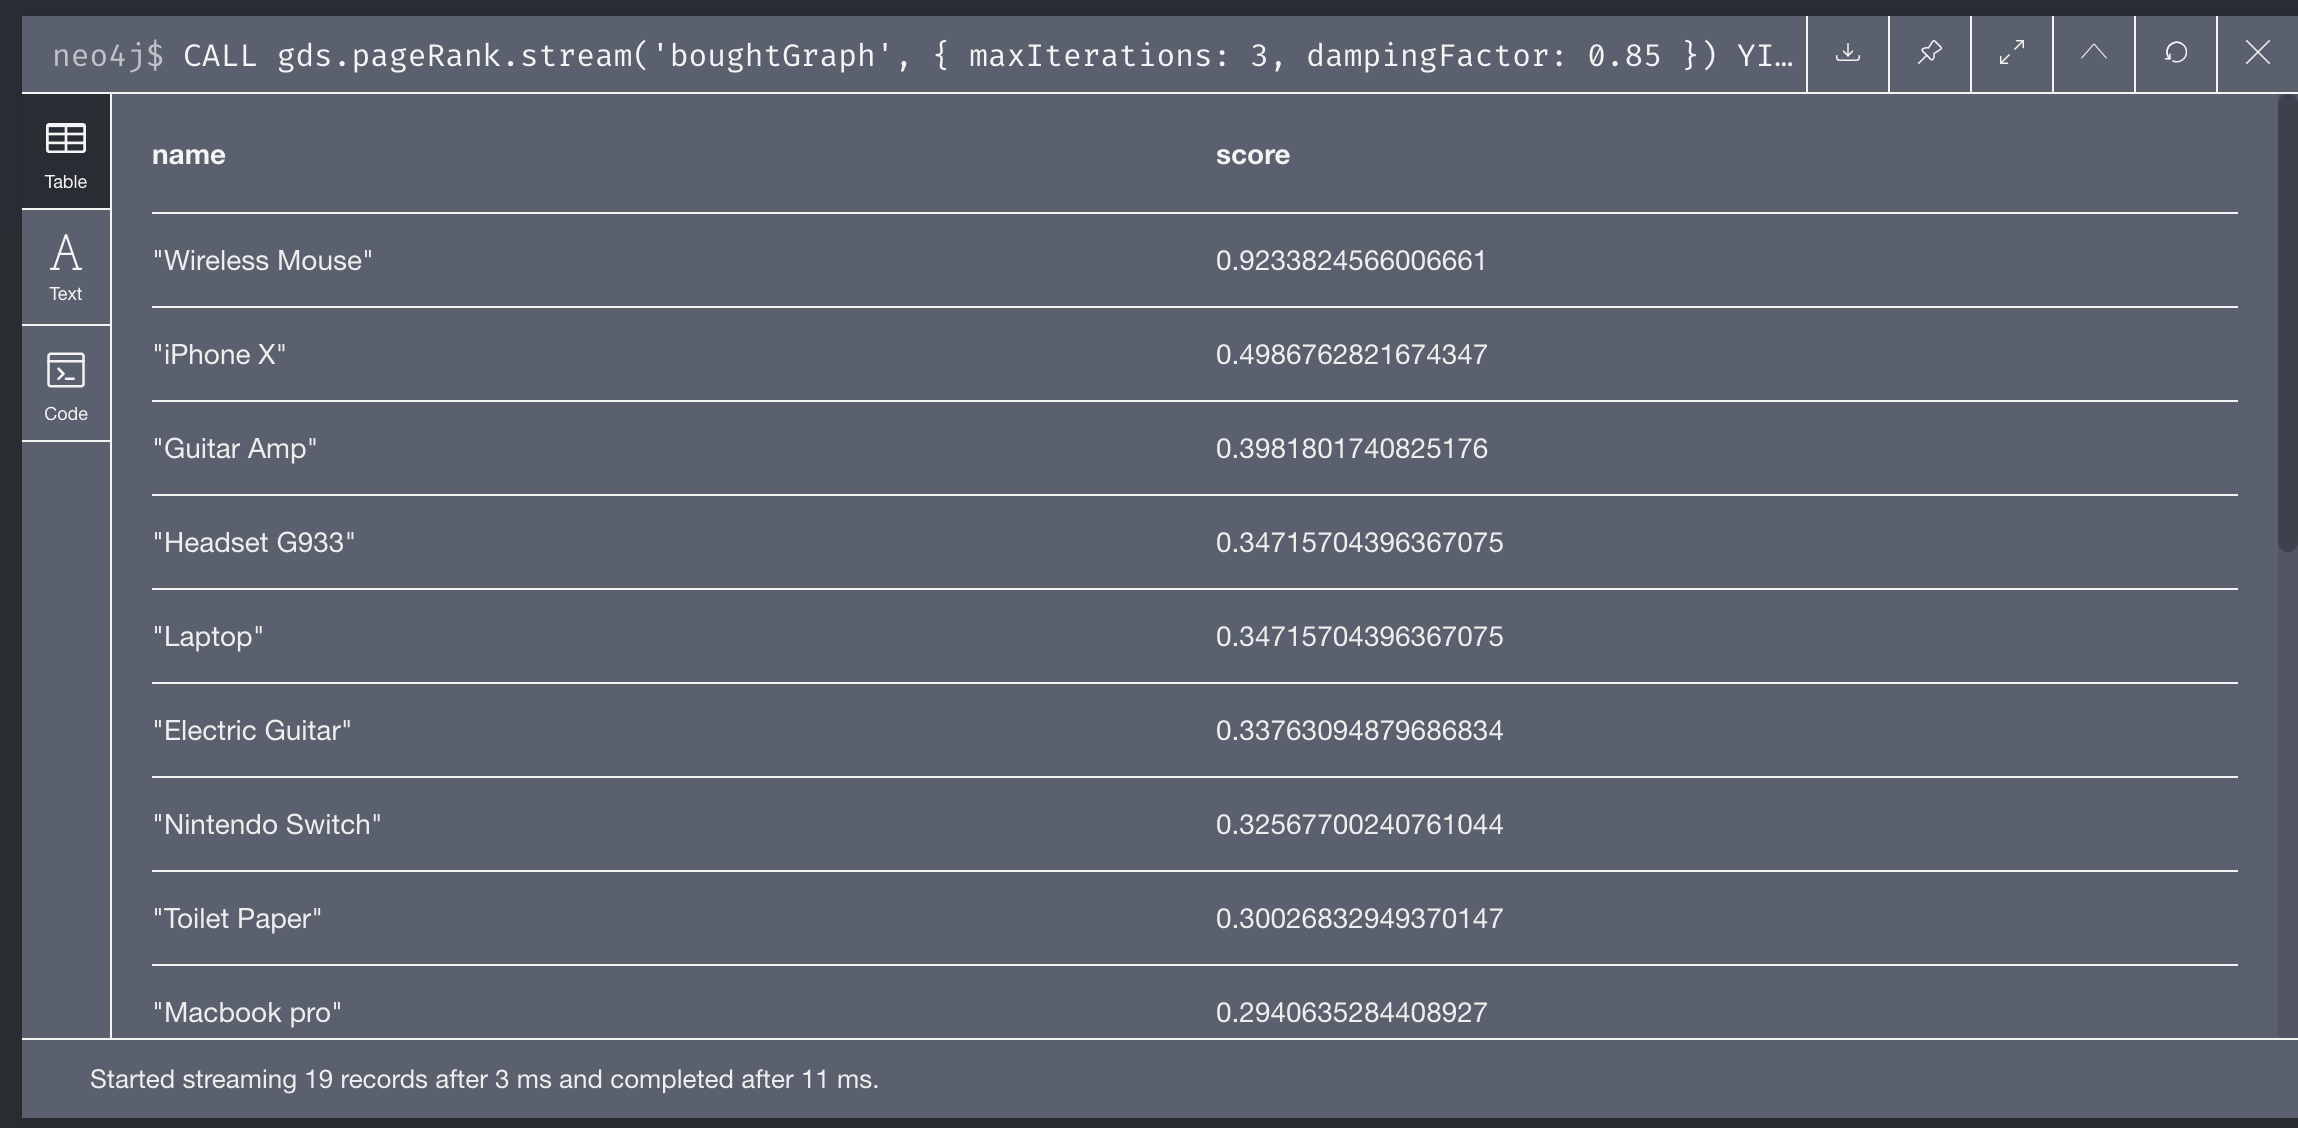
\includegraphics[width=0.95\textwidth]{img/pageRank_res_1}
	\caption{Resultaat PageRank algoritme}
	\label{fig:simplePageRankResult}
\end{figure}

\newpage
\subsection{Personalized PageRank}
\label{sec:Personalized PageRank}

Om de resultaten te baseren vanuit een bepaald startpunt, bijvoorbeeld een Customer, kan er een variant op PageRank gebruikt worden. Het algoritme zal dan starten in een bepaalde knoop (de gebruiker in kwestie) en zal op deze manier de meest relevante knopen vinden.

We gebruiken opnieuw de genoemde graaf uit de simpele PageRank, en voeren daar volgend algoritme op uit: 

\begin{lstlisting}[caption={Personalized PageRank algoritme }]
MATCH (c1:Customer {name: 'Tony'})
CALL gds.pageRank.stream('boughtGraph', {
	maxIterations: 1,
	dampingFactor: 0.85,
	sourceNodes: [c1]
	})
YIELD nodeId, score
RETURN gds.util.asNode(nodeId).name AS name, score
ORDER BY score DESC, name ASC
\end{lstlisting}

In het resultaat van deze query (Figuur \ref{fig:personalizedPageRankResult}) zien we dat de resultaten voor deze gebruiker in dezelfde lijn lopen als de algemene resultaten, maar dat er toch enkele producten bovenaan de lijst te vinden zijn die bij het gewone PageRank algoritme niet aan bod komen.

\begin{figure} [ht]
	\centering
	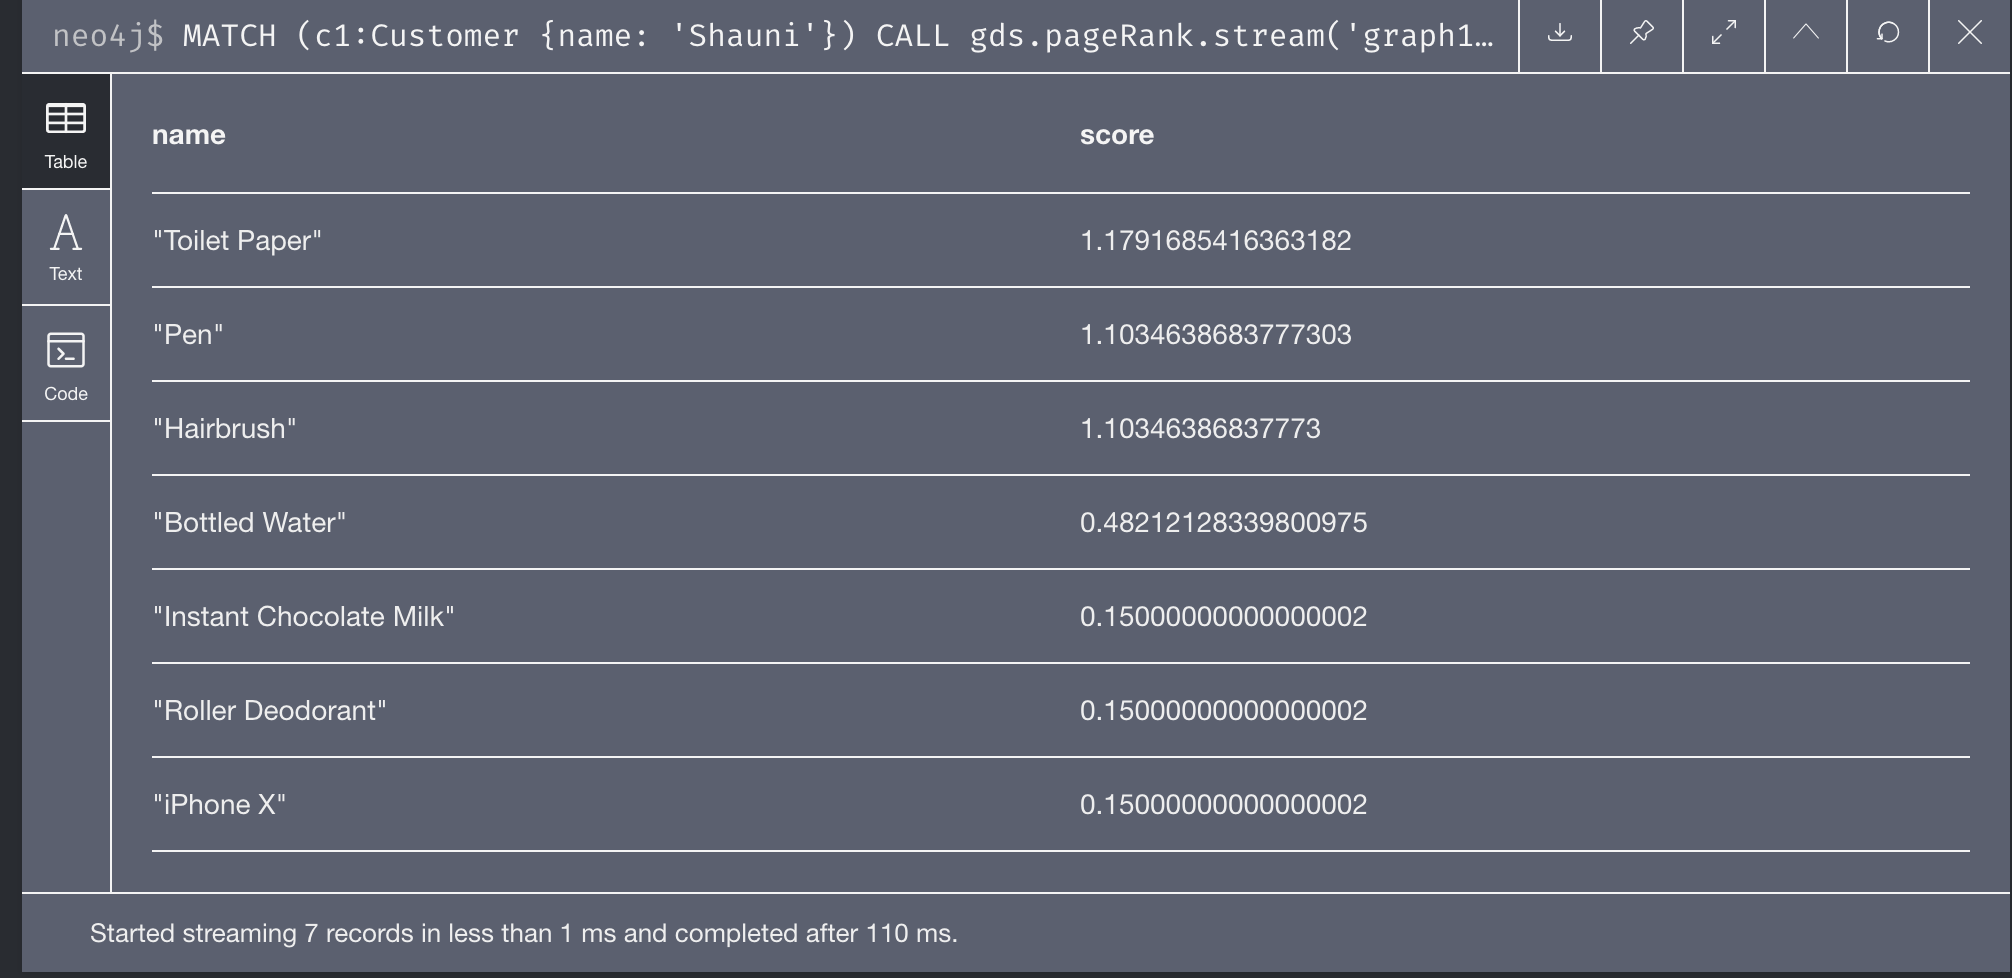
\includegraphics[width=0.95\textwidth]{img/persPageRank_res_1}
	\caption{Resultaat Personalized PageRank algoritme}
	\label{fig:personalizedPageRankResult}
\end{figure}

\newpage
\subsection{Community Detection}
\label{subsec: Community Detection}

Door het analyseren van de graaf met een community detection-algoritme kunnen groepen van gelijkaardige producten ontdekt worden. Op deze manier kan ontdekt worden welke gebruikers geïnteresseerd zijn in bepaalde groepen van producten, en kunnen er op basis van deze clusters aanbevelingen voorgesteld worden. 

Een nadeel aan deze techniek is dat deze last heeft van het cold-start probleem. Met andere woorden dat voor nieuwe gebruikers of producten, waarvoor dus nog niet bekend is tot welke cluster ze behoren of in welke clusters zij interesse hebben, nog geen correcte aanbevelingen kunnen bepaald worden.

Een voorbeeld van een community detection algoritme is het Louvain algoritme. De genoemde graaf van de uitwerking van PageRank zal opnieuw worden gebruikt voor dit algoritme.

\begin{lstlisting}[caption={ Louvain algoritme }]
CALL gds.louvain.stream('boughtGraph')
YIELD nodeId, communityId, intermediateCommunityIds
RETURN gds.util.asNode(nodeId).name AS name, communityId, intermediateCommunityIds
ORDER BY communityId DESC
\end{lstlisting}

Uit de resultaten worden enkele clusters ontdekt, deze zijn aangeduid op Figuur \ref{fig:LouvainResult}.

\begin{figure} [ht]
	\centering
	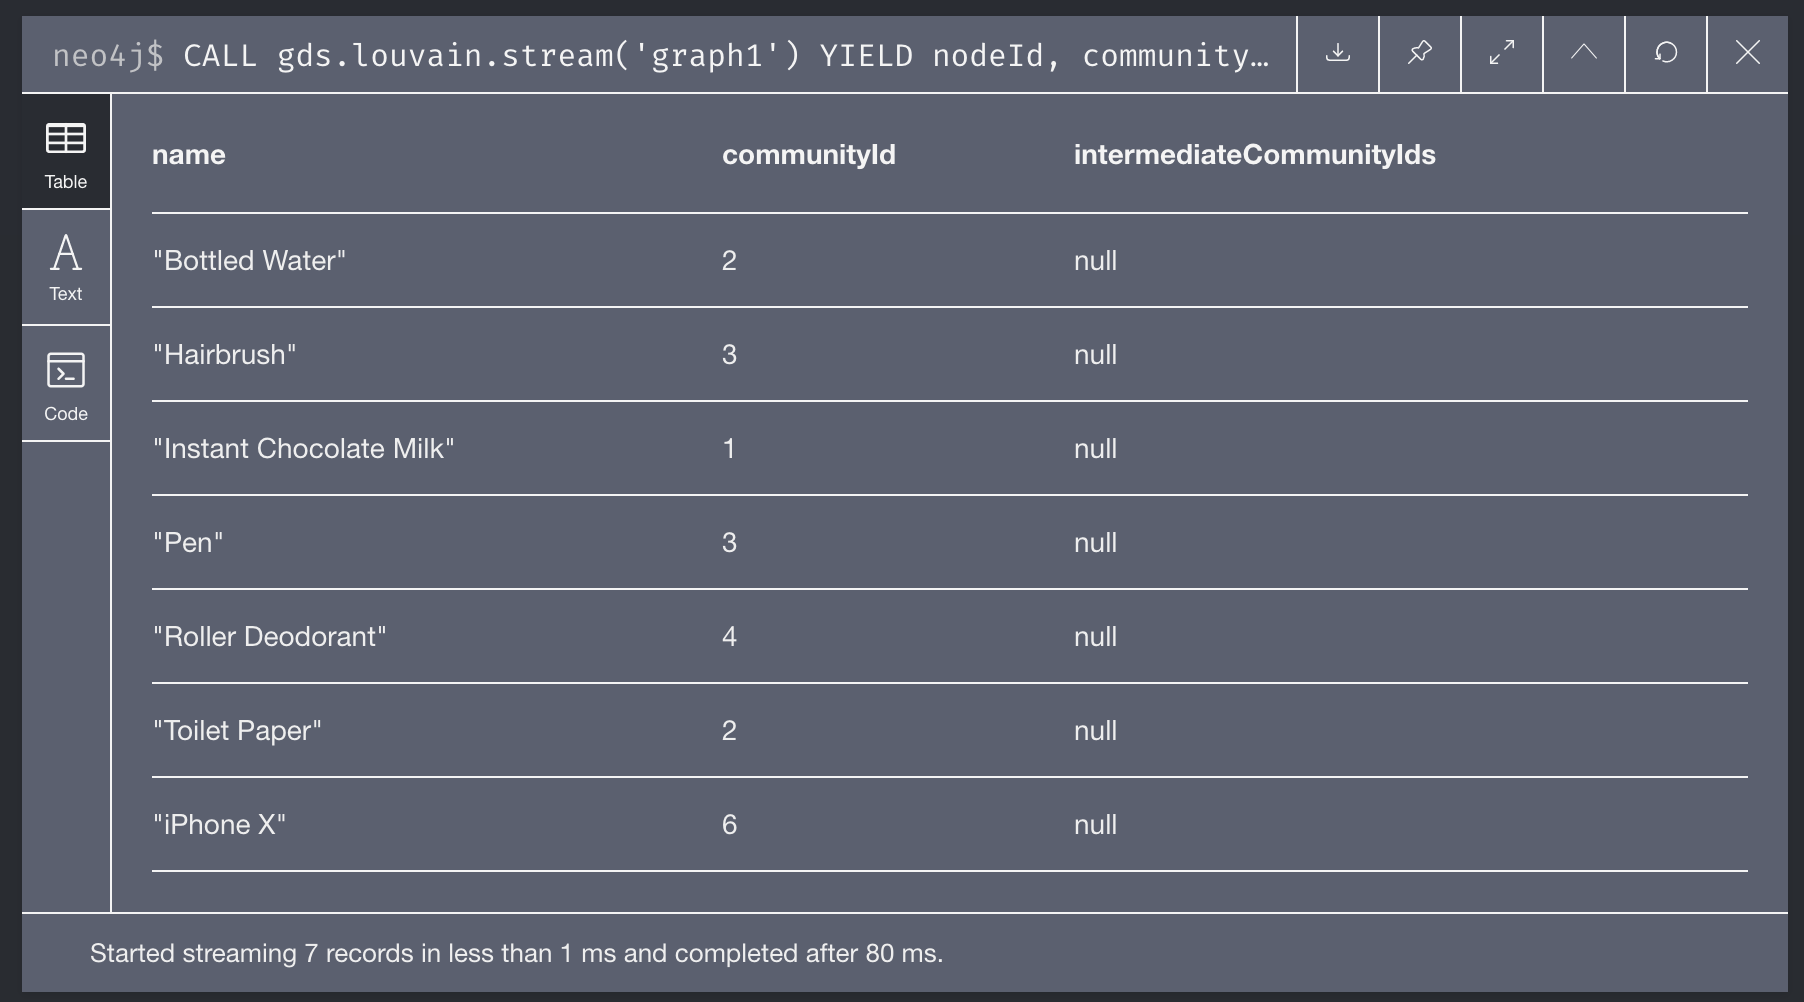
\includegraphics[width=0.95\textwidth]{img/Louvain_result}
	\caption{Resultaat Louvain algoritme}
	\label{fig:LouvainResult}
\end{figure}



